% !TEX TS-program = pdflatex
% !TEX encoding = UTF-8 Unicode

% This is a simple template for a LaTeX document using the "article" class.
% See "book", "report", "letter" for other types of document.

\documentclass[11pt]{article} % use larger type; default would be 10pt

%\usepackage[utf8]{inputenc} % set input encoding (not needed with XeLaTeX)
\usepackage[T1]{fontenc}
\usepackage{fixltx2e}
\usepackage{graphicx}
\usepackage{longtable}
\usepackage{float}
\usepackage{wrapfig}
\usepackage{soul}
\usepackage{textcomp}
\usepackage{marvosym}
\usepackage{wasysym}
\usepackage{latexsym}
\usepackage{amssymb}
\usepackage{hyperref}
\usepackage{caption}
\usepackage{pdfpages}
\usepackage{float}
%\usepackage[usenames, dvipsnames]{color}
\usepackage{listings}
\usepackage{xcolor}
\usepackage{subfig}
\usepackage{algpseudocode}
\usepackage[Algoritam]{algorithm}
\usepackage{amssymb}

%%% Examples of Article customizations
% These packages are optional, depending whether you want the features they provide.
% See the LaTeX Companion or other references for full information.

%%% PAGE DIMENSIONS
\usepackage{geometry} % to change the page dimensions
\geometry{a4paper} % or letterpaper (US) or a5paper or....
% \geometry{margin=2in} % for example, change the margins to 2 inches all round
% \geometry{landscape} % set up the page for landscape
%   read geometry.pdf for detailed page layout information

\usepackage{graphicx} % support the \includegraphics command and options

% \usepackage[parfill]{parskip} % Activate to begin paragraphs with an empty line rather than an indent

%%% PACKAGES
\usepackage{booktabs} % for much better looking tables
\usepackage{array} % for better arrays (eg matrices) in maths
\usepackage{paralist} % very flexible & customisable lists (eg. enumerate/itemize, etc.)
\usepackage{verbatim} % adds environment for commenting out blocks of text & for better verbatim
\usepackage{subfig} % make it possible to include more than one captioned figure/table in a single float
% These packages are all incorporated in the memoir class to one degree or another...

%%% HEADERS & FOOTERS
\usepackage{fancyhdr} % This should be set AFTER setting up the page geometry
\pagestyle{fancy} % options: empty , plain , fancy
\renewcommand{\headrulewidth}{0pt} % customise the layout...
\lhead{}\chead{}\rhead{}
\lfoot{}\cfoot{\thepage}\rfoot{}

%%% SECTION TITLE APPEARANCE
\usepackage{sectsty}
\allsectionsfont{\sffamily\mdseries\upshape} % (See the fntguide.pdf for font help)
% (This matches ConTeXt defaults)

%%% ToC (table of contents) APPEARANCE
\usepackage[nottoc,notlof,notlot]{tocbibind} % Put the bibliography in the ToC
\usepackage[titles,subfigure]{tocloft} % Alter the style of the Table of Contents
\renewcommand{\cftsecfont}{\rmfamily\mdseries\upshape}
\renewcommand{\cftsecpagefont}{\rmfamily\mdseries\upshape} % No bold!

%%% END Article customizations

%%% The "real" document content comes below...

\title{Teorija}
\author{Filip Paveti\'{c}}
%\date{} % Activate to display a given date or no date (if empty),
         % otherwise the current date is printed 

\begin{document}
\maketitle

\section{LCS kao nositelj informacija za alignment kod duga\v{c}kih readova}

\v{Z}elim pokazati da je za duga\v{c}ke readove LCS dobra metrika za smje\v{s}tanje readova na referentni genom. Preciznije, pokazat \'{c}e se da je za duge readove mala vjerojatnost da se postigne veliki LCS na random mjestu u genomu. Dugi read modeliramo kao slu\v{c}ajan string u kojem se svaka od baza pojavljuje s vjerojatnostima danima u tablici 1.

\begin{table}[H]
\centering
\begin{tabular}{|c||c|c|c|c|c|c|}
\hline
	Baza & Vjerojatnost\\
\hline
\hline
	A & 0.30\\
\hline
	C & 0.20\\
\hline
	G & 0.20\\
\hline
	T & 0.30\\
\hline
\end{tabular}
\caption{Vjerojatnosti pojavljivanja pojedine baze - $p_{baza}$}
\end{table}

\subsection{Smje\v{s}tanje reada na genom, uz $k=1$ (seedovi su nam duljine 1)}

Trenutno promatram slu\v{c}aj idealnog ra\v{c}unanja LCS-a, u sljede\'{c}oj sekciji \'{c}u gledati koliko gubimo kada duljinu seeda po\v{c}nemo pove\'{c}avati. Ono \v{s}to znamo je da ve\'{c}ina reada i njegove to\v{c}ne pozicije na genomu dolazi uslijed gre\v{s}aka kod ocitanja. Ta je gre\v{s}ka unaprijed poznata. Ona je konstantna na svakoj poziciji reada. Ozna\v{c}ujemo je sa $p_{error}$. U ovim analizama sada gledam samo supstitucijsku gre\v{s}ku, mogu kasnije pro\v{s}iriti i na indele, ne bi se trebalo ni\v{s}ta zna\v{c}ajno promijeniti.

\begin{figure}[H]
  \centering
    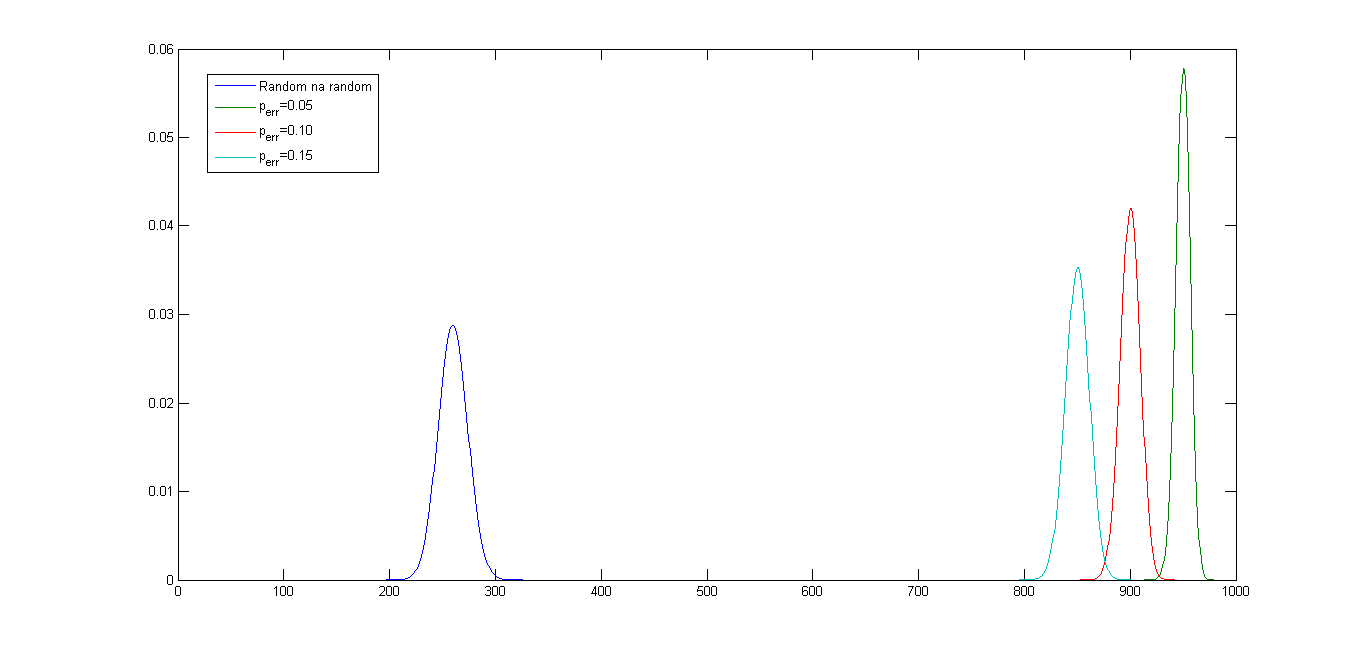
\includegraphics[width=1\textwidth]{lcs_k1.png}
  \caption{Random na random linija prikazuje distribuciju LCS-ova dva random fragmenta genoma. Ostale linije prikazuju distribucije LCS-a izmedju random fragmenta genoma i njegove kopije u koju je uneseno $p_{err}$ supstitucijske gre\v{s}ke.}
\end{figure}

Iz grafova se vidi da kada ra\v{c}unamo savr\v{s}en LCS ($k=1$), vjerojatnost da random string postigne dobar LCS score je zanemariva.

\subsection{\v{S}to kada pove\'{c}amo duljinu seeda?}

\begin{figure}[H]
  \centering
    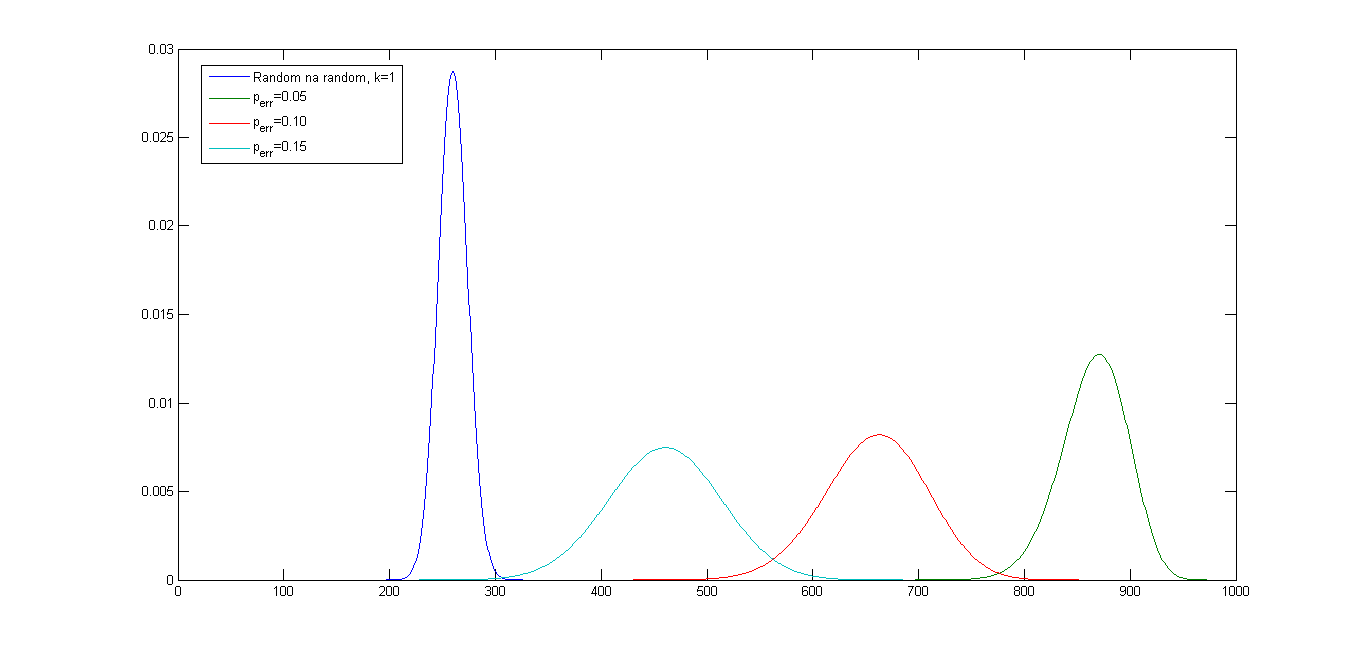
\includegraphics[width=1\textwidth]{lcs_k10.png}
  \caption{Ovdje je duljina seeda 10. Random na random linija prikazuje distribuciju LCS-ova dva random fragmenta genoma. Ostale linije prikazuju distribucije LCS-a izmedju random fragmenta genoma i njegove kopije u koju je uneseno $p_{err}$ supstitucijske gre\v{s}ke.}
\end{figure}

Pove\'{c}avanjem seeda na 10 vi\v{s}e nemamo jako veliku marginu izmedju scorova random stringova i onih koji su sli\v{c}ni. Slu\v{c}aj kad je $p_{err}=0.15$ izgleda kao grani\v{c}ni.

\begin{figure}[H]
  \centering
    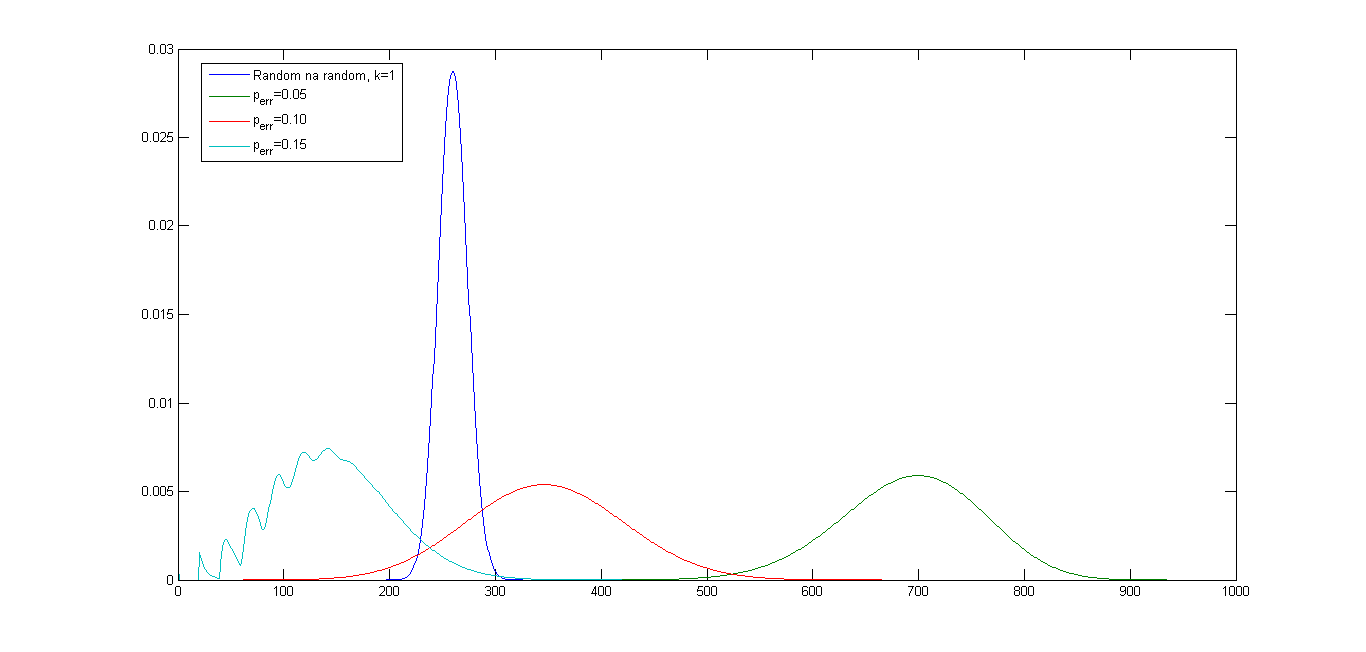
\includegraphics[width=1\textwidth]{lcs_k20.png}
  \caption{Ovdje je duljina seeda 20. Random na random linija prikazuje distribuciju LCS-ova dva random fragmenta genoma. Ostale linije prikazuju distribucije LCS-a izmedju random fragmenta genoma i njegove kopije u koju je uneseno $p_{err}$ supstitucijske gre\v{s}ke.}
\end{figure}

Kod duljine seeda 20 izgleda da teoretski ne pali ovo, osim za mali postotak gre\v{s}ke ($p_{err}=0.05$). To nam je i vidljivo na preciznosti koju dobivamo za veliku gre\v{s}ku u LISA-i (a ona je usporediva s ostalim alignerima).


\end{document}
